\subsection{Object Models}
  \label{subsection:model}

  This chapter describes the design of the object models used by the business layer. The essential object models of the system can be defined by revisiting the sequences listed on \autoref{subsection:controller} and identifying the important structures needed to fulfill the requirements.
  
  \subsubsection{Validation Rule}
    \label{subsub:rule}

    A validation rule is a structure of information used in a validation process by supplying the FDS the necessary information to make an HTTP request to an external endpoint and evaluating its response, affecting the overall fraud score of a validation process through its evaluation result. Through a detailed analysis of the sequence illustrated on \autoref{fig:notif-sequence}, it is essential that the \emph{validation rule} model contains the following attributes:

    \begin{itemize}
      \item A URL pointing to an external endpoint
      \item A list of conditions to evaluate the response returned by the external endpoint
      \item A unique identifier
      \item A fail score, which determine the severity of the rule if the evaluation failed
    \end{itemize}

    It might also be necessary to have an identifier in the validation rule to skip its evaluation in certain cases. Other than that, as the FDS would make an HTTP request to an external endpoint based on the information listed on a validation rule, the following attributes are needed to provide a more robust configuration:

    \begin{itemize}
      \item HTTP method 
      \item Request header fields
      \item Request body
    \end{itemize}

    As the FDS interacts with external endpoints, there is no guarantee that the external endpoint will always be accessible. An additional attribute to specify and configure a retry strategy in such cases can be useful. However, a retry strategy can be really specific to its implementation and therefore will be discussed in \autoref{impl_model:rule__retry}.

    An additional \verb;priority; attribute is also provided to enable the possibility to run rule validations according to its priority order.

    \begin{figure}[!ht]
      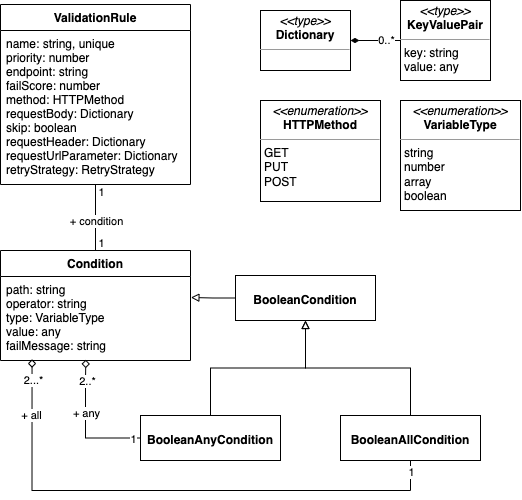
\includegraphics[width=0.8\textwidth]{diagrams/entity-validationrule.png}
      \caption{UML diagram of the validation rule model}
      \label{fig:uml_validation_rule}
    \end{figure}
    
    The \verb;condition; attribute plays an important role for a validation rule, as it defines how the response returned by the external endpoint should be structured to pass a rule evaluation. It is intended to design the condition attribute to be robust and configurable. The \verb;path; of a condition defines a JSONPath\autocite{Friesen2019} expression to access information available of the current validation scope, such as customer information or response returned by the external endpoint. The \verb;type; attribute of a condition determines the data type of the attribute accessed by the \verb;path; attribute. The \verb;type; attribute also determines which operators are available to use\footnote{For example: a condition with \emph{type} "string" cannot use the "incl" \emph{operator}, because the "incl" \emph{operator} is only available for "array" \emph{type}.}. The \verb;operator; attribute refers to a name of operator to be used to evaluate the condition (for example: "eq", "incl") by comparing the property accessed by \verb;path; attribute with the value of the \verb;value; attribute. The available operator names are predefined and restricted to the condition's type attribute. More information regarding operators will be discussed in \autoref{impl_cl:op}. The \verb;failMessage; attribute of a condition refers to a message that is going to be appended to the validation result's \verb;messages; attribute after a validation is completed, if the corresponding rule evaluation failed.

    \newpage
    \begin{lstlisting}[caption={Validation rule example (JSON)}, language=json]
{
  "name": "Example",
  "skip": false,
  "priority": 2,
  "endpoint": "http://localhost:8000/validate",
  "method": "GET",
  "failScore": 0.7,
  "condition": {
    "path": "$.response.statusCode",
    "type": "number",
    "operator": "eq",
    "value": 200,
    "failMessage": "Status code doesn't equal to 200"
  },
  "requestUrlParameter": {},
  "requestBody": {},
  "requestHeader": {}
}
    \end{lstlisting}

    A validation rule might contain more than a single condition to pass an evaluation. In such cases, the user needs to define how to determine whether an evaluation should pass: either pass an evaluation if \textbf{ALL} the conditions is true or pass an evaluation if \textbf{AT LEAST ONE (ANY)} of the conditions is true. This can be achieved by having the \verb;condition; attribute as an object with a single attribute, either \emph{all} or \emph{any} and an array of conditions as the attribute's value.

    \begin{lstlisting}[caption={Validation rule \textbf{condition} attribute example with ALL condition (JSON)}, language=json]
{
  "condition": {
    "all": [
      {
        "path": "$.response.statusCode",
        "type": "number",
        "operator": "eq",
        "value": 200,
        "failMessage": "Status code doesn't equal to 200"
      },
      {
        "path": "$.response.body.valid_address",
        "type": "boolean",
        "operator": "eq",
        "value": false,
        "failMessage": "Address is invalid"
      }
    ]
  }
}
\end{lstlisting}

    \newpage
    \begin{lstlisting}[caption={Validation rule \textbf{condition} attribute example with ANY condition (JSON)}, language=json]
{
  "condition": {
    "any": [
      {
        "path": "$.response.statusCode",
        "type": "number",
        "operator": "eq",
        "value": 200,
        "failMessage": "Status code doesn't equal to 200"
      },
      {
        "path": "$.response.body.valid_address",
        "type": "boolean",
        "operator": "eq",
        "value": false,
        "failMessage": "Address is invalid"
      }
    ]
  }
}
    \end{lstlisting}

  \subsubsection{Validation Result}

    A validation result is the result of a validation process. A validation result contains a resulting fraud score, which is the probability of a certain customer being a fraud. The algorithm to calculate the fraud score will be discussed as part of the \autoref{impl_cl:flow}.
    By evaluating the sequences listed on \autoref{fig:regis-sequence} and \autoref{fig:notif-sequence}, the following attributes are needed:

    \begin{itemize}
      \item A unique validation ID
      \item A fraud score 
    \end{itemize}

    Furthermore, information regarding the total checks, run checks, and additional information that contains the start and end date of the validation process as well as the customer information used for the validation are essential. The customer information is generic, and the system should be able to do a validation process regardless of its structure. The validation result should also return a list of validation rule names, whose evaluations are skipped due to its \verb;skip; attribute being set to \verb;true;.

    Even though the resulting fraud score determines the probability of a customer being a fraud, it is also important to further analyze the actual evaluation result of each validation rule. For example, a certain action can be run if the evaluation of a specific rule failed or the information regarding the rule evaluations can also be used to display the current progress of a validation process (implementation of this specific functionality will be discussed more in \autoref{impl_sse}). 

    To provide such information on a validation result, the \verb;events; attribute will be introduced, which refers to rule evaluation events within a validation process. A rule evaluation event should contain the following attributes:

    \begin{itemize}
      \item Unique identifier of the event (name of the rule being evaluated)
      \item Status of the event (not started, failed, passed or running) 
      \item If available, start date of a rule evaluation event 
      \item If available, end date of a rule evaluation event 
      \item A list of messages, containing error messages of an evaluation event
    \end{itemize}

    \begin{figure}[!ht]
      \centering
      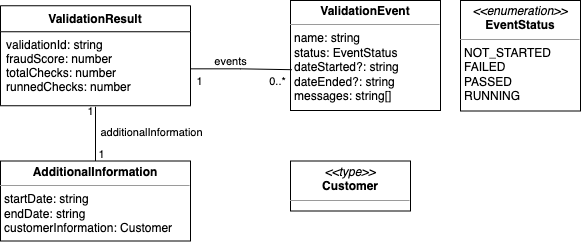
\includegraphics[width=0.8\textwidth]{diagrams/entity-validationresult.png}
      \caption{UML diagram of the validation result model}
      \label{fig:uml_validation_result}
    \end{figure}
    
    \begin{lstlisting}[caption={Validation result example (JSON)}, language=json]
{
  "validationId": "3112dc4a-45f5-41b8-883a-715dcbe9a490",
  "totalChecks": 3,
  "runnedChecks": 2,
  "skippedChecks": [
    "Skip rule",
  ],
  "additionalInfo": {
    "startDate": "2022-06-12T09:16:24.618Z",
    "customerInformation": {}
  },
  "events": [
    {
      "name": "User's email domain is not blacklisted",
      "status": "PASSED",
      "dateStarted": "2022-06-12T09:16:34.694Z",
      "dateEnded": "2022-06-12T09:16:39.725Z",
      "messages": []
    },
    {
      "name": "User's email is not blacklisted",
      "status": "FAILED",
      "dateStarted": "2022-06-12T09:16:39.725Z",
      "dateEnded": "2022-06-12T09:16:44.756Z",
      "messages": [
        "User's email is blacklisted!"
      ]
    }
  ],
  "fraudScore": 0.425  
}
    \end{lstlisting}